\documentclass[pdflatex,sn-mathphys-num]{sn-jnl}
\usepackage{graphicx,amsmath,amssymb,booktabs,tabularx,url,microtype,etoolbox,placeins,flafter,needspace}
\raggedbottom
\AtBeginDocument{\let\burl\url}
\makeatletter
% Keep the complete structured abstract together without changing type sizes.
\patchcmd{\@maketitle}{\vskip21pt}{\vskip0pt}{}{\errmessage{Title spacing patch failed}}
\patchcmd{\@maketitle}{\vskip20pt}{\vskip0pt}{}{\errmessage{Article-title spacing patch failed}}
\patchcmd{\@maketitle}{\vskip20pt}{\vskip4pt}{}{\errmessage{Author spacing patch failed}}
\patchcmd{\abstracthead}{-22pt}{-8pt}{}{\errmessage{Abstract spacing patch failed}}
\patchcmd{\@maketitle}{\vskip24pt}{\vskip0pt}{}{\errmessage{Address spacing patch failed}}
\patchcmd{\@maketitle}{\vskip24pt}{\vskip0pt}{}{\errmessage{Email spacing patch failed}}
\def\ps@paper{\let\@oddhead\@empty\let\@evenhead\@empty
  \def\@oddfoot{\hfil\thepage\hfil}\let\@evenfoot\@oddfoot}
\let\ps@titlepage\ps@paper
\let\ps@headings\ps@paper
\makeatother
\pagestyle{paper}
% All numerical claims are expanded into generated fragments.

\begin{document}
\title[Crowd-label supervision for selective FER]{Evaluating Crowd-Label Supervision for Selective Facial-Expression Recognition}
\author[1]{\fnm{Gunjan Kumar} \sur{Mishra}}\email{mgunjan67@gmail.com}
\author[2]{\fnm{Bijaya} \sur{Ghimire}}\email{vijay.gh74@gmail.com}
\author*[3]{\fnm{Badri Raj} \sur{Lamichhane}}\email{d6622300231@g.siit.tu.ac.th}
\author[4]{\fnm{Alan} \sur{Shah}}\email{shahalan0202@gmail.com}
\affil[1]{\orgname{WorldQuant University}, \orgaddress{\city{Washington, D.C.}, \country{United States}}}
\affil[2]{\orgdiv{Department of Electronics and Computer Engineering}, \orgname{Institute of Engineering, Paschimanchal Campus}, \orgaddress{\city{Pokhara}, \country{Nepal}}}
\affil*[3]{\orgdiv{School of Information, Computer and Communication Technology}, \orgname{Sirindhorn International Institute of Technology, Thammasat University}, \orgaddress{\city{Pathum Thani}, \country{Thailand}}}
\affil[4]{\orgname{Herald College Kathmandu}, \orgaddress{\city{Kathmandu}, \country{Nepal}}}
\abstract{\noindent\textbf{Purpose:} Facial-expression annotations can contain disagreement that is lost when training uses a single label. This study examines whether distribution-based supervision improves predictions when a classifier reports only its most confident decisions.
\par\smallskip
\noindent\textbf{Methods:} We compared five Swin-T training targets on FER2013 with FER+ annotations, using three paired seeds and secondary ResNet-18 comparisons. Controls preserved dominant target probabilities or tied maxima. The primary outcome was mean annotation disagreement---the fraction of votes inconsistent with the predicted category---among the 80\% most confident predictions. Additional analyses examined distributional agreement, identical accepted images, and calibration transfer. Evaluation retained categories outside the seven outputs. Frozen models were evaluated on 1,440 RAVDESS clips.
\par\smallskip
\noindent\textbf{Results:} For validation-selected Swin-T, distributional supervision reduced disagreement from 24.06\% to 23.68\% relative to the uniform-minority control; the reduction relative to hard targets was 2.61 percentage points. The corresponding ResNet-18 comparison instead increased disagreement by 0.17 percentage points. Distributional supervision nevertheless achieved lower squared distance than both softening controls in every tested seed, backbone and checkpoint state. Comparisons on identical accepted images depended on which model selected them. External comparisons varied with seed, checkpoint and annotation reference. All 36 nonempty empirical calibration-transfer settings exceeded their risk targets on testing.
\par\smallskip
\noindent\textbf{Conclusion:} In these experiments, improved agreement with crowd-label distributions did not consistently improve confidence-selected category predictions. Selective performance must therefore be interpreted in relation to the accepted images and annotation vocabulary.
}
\keywords{facial-expression recognition, crowd annotations, selective prediction, label distributions, supported vote mass, confidence calibration}
\maketitle

\section{Introduction}
Facial-expression recognition (FER) is commonly formulated as predicting a category from a face image, but multiple annotators need not assign the same category. FER+ records this variation by associating FER2013 images with distributions of human responses rather than relying exclusively on the original categorical labels \cite{goodfellow2013fer,barsoum2016ferplus}. Distribution-based supervision retains the relative frequency of these responses and has been investigated as an alternative to hard-label training \cite{barsoum2016ferplus,washington2021crowdsourcing}. Agreement with a response distribution and agreement with a categorical reference are nevertheless different evaluation objectives. This distinction becomes important when a classifier is allowed to withhold predictions rather than assign a category to every image.

Selective prediction evaluates the trade-off between the proportion of inputs accepted and the disagreement or error among the accepted predictions \cite{geifman2017selective,geifman2019selectivenet}. Here, coverage denotes the fraction of images accepted, and disagreement is the mean fraction of annotations that do not match the predicted category. Two models evaluated at the same coverage may accept different images. Their selective risks can therefore differ because they make different category predictions, because they select different images, or because both change. A comparison using each model's own confidence ranking does not, by itself, distinguish these possibilities. A probability vector can also move closer to the annotation distribution without changing its most probable category, so distributional agreement and category disagreement need not improve together.

The choice of training control creates a second interpretive difficulty. Replacing a hard target with an empirical vote distribution changes both the probability assigned to the dominant category and the allocation of probability among the remaining categories. An advantage over hard-label training consequently does not isolate the contribution of the observed minority-category allocation. We examine this comparison using controls that preserve the dominant target probability while redistributing the remaining probability, together with controls that account for tied maxima. All conditions within a backbone and random seed retain the same training images, weights derived from votes for the model's output categories, architecture, initialization, sample order, augmentation, and optimization budget. The largest training-target probability describes the annotations, whereas prediction confidence is computed from the fitted model. The comparisons concern specified target representations; the softening controls do not additionally match target entropy or aggregate class proportions.

The annotation vocabulary introduces a further distinction between training and evaluation. FER+ includes contempt, unknown, and not-a-face responses in addition to the seven categories predicted by the models examined here \cite{barsoum2016ferplus}. We call categories in the model's output vocabulary supported categories. Votes for the other categories cannot be matched by a seven-category prediction. They therefore contribute to disagreement even when the model chooses the most strongly supported category available to it. Restricting the evaluation to supported votes would change the reference against which the model is scored. We instead retain the complete annotation distribution and distinguish unsupported vote mass, ambiguity among supported categories, and disagreement beyond the best available supported-category prediction.

This study brings these issues together in a matched empirical evaluation on FER2013 with FER+ annotations. The primary follow-up comparison uses validation-selected Swin-T models at 80\% coverage across three paired training seeds. ResNet-18, distributional distance, fixed-epoch checkpoints, identical-image comparisons, confidence-score sensitivity and calibration transfer retain the secondary or exploratory roles specified in Sect.~3.1. The analysis addresses three research questions:
\begin{enumerate}
\item \textbf{RQ1: Target representation.} How do observed crowd targets compare with controls that preserve the highest target probability or tied maxima, under the same training protocol?
\item \textbf{RQ2: Interpretation.} How does the comparison change when models accept identical images, and when we account for the annotation reference and categories absent from the model?
\item \textbf{RQ3: Robustness and transfer.} Which findings hold across the tested backbones, confidence scores, saved model states (checkpoints), calibration transfer and external clips?
\end{enumerate}

The results show why these comparisons need to be considered together. The selective advantage of empirical-distribution supervision over hard targets becomes smaller when the dominant target probability is preserved by the control. Although distributional agreement improves across the tested within-source configurations, the selective advantage does not persist across both backbones, and comparisons on identical accepted images depend on the selecting model. Frozen evaluation on 1,440 RAVDESS clips \cite{livingstone2018ravdess} and calibration-to-test transfer further examine how the conclusions depend on the scoring reference and achieved operating point. The contribution is a controlled account of these dependencies, using established learning architectures rather than a new recognition or rejection algorithm. Section~5 develops the implications for evaluating selective predictions.

A sender-controlled messaging prototype motivated the seven-category implementation. Related applications include text-based notifications in EmotionPush \cite{wang2016emotionpush}, facial and textual signals in EmoChat \cite{chong2019emochat}, and expression-informed emoji selection \cite{liu2019selfawareness}. Agreement with expression annotations should not be equated with a person's internal emotion, intention, or sincerity \cite{barrett2019emotions}. The prototype and its unvalidated communication role are therefore documented separately in the supplement. The empirical conclusions concern annotation-based facial-expression evaluation.


\section{Related work}
\subsection{Facial-expression supervision}
FER+ compares hard-label with distribution-based training using multiple annotations for FER2013 images \cite{barsoum2016ferplus}. Washington et al. extend the study of human response distributions using hard- and soft-target ResNet-152 models on CAFE, distinguishing categorical-reference performance from distributional agreement \cite{washington2021crowdsourcing}. These studies establish distribution-based supervision and the possibility that categorical and distributional measures favor different models. Our study examines that relationship under controls preserving the largest target probability or tied maxima, with selective comparisons on identical accepted images and explicit accounting for omitted response categories. Seven model outputs are retained for compatibility with the prototype, while evaluation uses all ten FER+ responses; this differs from the original eight-expression FER+ benchmark.

Methods for uncertain expression labels differ in how they use disagreement. Self-Cure Network combines weighting and relabeling \cite{wang2020scn}, whereas Le et al. construct uncertainty-aware targets using neighbors in valence--arousal space \cite{le2023uncertainty}. MIDAS extends mixup to soft-labeled facial-expression videos \cite{kawamura2024midas}. Here, observed static-image votes remain fixed and only their training-target representation changes. This design examines a supervision comparison rather than the additional mechanisms used by those methods, whose reported benchmark scores use different protocols.

The feature extractors and channel gates also follow established designs. Swin Transformer provides hierarchical shifted-window features \cite{liu2021swin}, and the gate uses the squeeze-and-excitation principle \cite{hu2018senet}. Vats and Chadha describe a related combination of Swin and squeeze-and-excitation for FER (unpublished preprint, 2023; \url{https://arxiv.org/abs/2301.10906}). Architecture is fixed within each backbone family so that the training target is the experimental variable; frozen transfer to acted speech videos then examines the external scope of the resulting comparisons.

\subsection{Selective prediction and annotation disagreement}
Selective classification studies the trade-off between rejection and error \cite{geifman2017selective}; SelectiveNet learns the rejector jointly with prediction \cite{geifman2019selectivenet}. In subjective language tasks, Crowd-Calibrator connects this trade-off to annotation disagreement \cite{khurana2024crowd}. It estimates crowd distributions from learned representations and uses their distance from model probabilities, optionally with predictive entropy, to decide whether to abstain. These approaches place rejection within the learning or calibration procedure. Our primary analysis instead compares supervision targets using maximum probability, with exploratory margin and negative-entropy scores applied to unchanged fitted models. It examines probability-only rankings rather than implementing or benchmarking a learned selector.

Calibration provides a related but distinct question because softmax scores need not be calibrated probabilities \cite{guo2017calibration}. Tao, Luo, Dong and Xu distinguish calibration against majority labels from calibration against annotator distributions and propose ambiguity-aware post-hoc calibrators (\emph{Confidence Calibration under Ambiguous Ground Truth}, unpublished preprint, 2026; \url{https://arxiv.org/abs/2603.22879}). This distinction motivates reporting distributional distance, equal-coverage category disagreement and calibration-fitted operating points separately. The present study measures those outcomes without implementing their calibrators; lower squared distance alone is not interpreted as calibrated deployment confidence, nor is an empirically fitted error target treated as a risk guarantee.

Recent dynamic-FER preprints combine several uncertainty sources. Yiming Wang, Frederick W. B. Li, and Jingyun Wang use a Dirichlet--multinomial vote-count objective, predicted disagreement, and a rejection score incorporating ambiguity, vacuity, temporal instability and input quality (\emph{Predicting Human Disagreement for Calibrated Dynamic Facial Expression Recognition}, unpublished preprint, 2026; \url{https://arxiv.org/abs/2609.17130}). The work was submitted to ICASSP 2027, with acceptance unverified. Inoshita and Ueno use a fine-tuned DINOv2 ensemble to estimate aleatoric and epistemic uncertainty, examining human disagreement and distribution shift before routing inputs (\emph{Interpretable Uncertainty Routing Separating Emotion Ambiguity from Distribution Shift in Facial Expression Recognition}, unpublished preprint, 2026; \url{https://arxiv.org/abs/2606.22725}). Our static-image controls and annotation-vocabulary accounting address a narrower measurement question without implementing these dynamic or ensemble methods. Because RAVDESS changes several factors together, the external evaluation is a frozen-pipeline stress test rather than a separation of intrinsic ambiguity from distribution shift. Differences in task, selector and reference definitions also prevent treating the cited language-task or dynamic-FER scores as directly comparable benchmarks.

\Needspace{8\baselineskip}
\section{Methods}
\subsection{Study design and analysis hierarchy}
The experiments compared alternative representations of the same crowd annotations while holding the training conditions fixed within each backbone and random seed. Swin-T was evaluated with hard labels, empirical supported-category vote distributions, and three controls addressing dominant probabilities or tied maxima. ResNet-18 provided secondary comparisons of the three distributional targets. Separate image roles were used for optimization, checkpoint selection, threshold calibration, and primary testing, with exact-pixel overlap removed between roles as described below. Evaluation addressed two distinct outcomes: disagreement of confidence-selected category predictions with the observed votes, and squared distance from the complete vote distribution. Comparisons on identical accepted-image sets examined whether the predictor ordering depended on which model selected the images. External evaluation applied frozen classifiers to RAVDESS clips without additional training. Across the within-source phases, 24 training runs produced 48 validation-selected and epoch-12 states; all 48 have recorded distributional scores and confidence-score summaries.

The within-source experiments comprise four adaptive phases: initial hard/soft runs, Uniform/Tie-hard controls, a Tie-Uniform control, and a ResNet-18 follow-up. Soft denotes the empirical supported-category vote target; Uniform preserves its dominant probability while spreading the remainder equally among the other categories. The tie-preserving controls are defined with the complete target construction below. Each phase was specified before training and frozen before its own calibration/test inference, but earlier outcomes were already known. In particular, earlier PrivateTest results informed the follow-up phases. The validation-selected Swin-T Soft-minus-Uniform contrast is the primary follow-up comparison. Tie-preserving controls, fixed-epoch checkpoints, distributional distance and ResNet analyses have the secondary roles described below. The complete secondary distribution-distance comparison was assembled from previously recorded values after outcomes were known. The subsequent confidence-score analysis reuses previously examined test predictions and remains exploratory even though its scores and reporting rules were fixed before the additional summaries were computed.

The external analysis followed a local protocol frozen before external model outcomes, after internal findings and RAVDESS annotation summaries were known. It is therefore not an external preregistration. A pre-analysis amendment corrected a swapped disgust/surprise response mapping against the primary source's descriptors and accuracy records before any external performance metric was computed. The original freeze and amendment are retained. External retained-output diagnostics were specified after the internal and external results were known and are exploratory. Supplementary Sect.~S9 and Online Resources 1 and 8 consolidate the phase-specific protocols, freeze records, amendment and execution metadata. Table~\ref{tab:phases} summarizes the adaptive phases.
\begin{table}[htbp]
\caption{Adaptive experimental phases on the same source; every phase uses seeds 17, 42, 89 and selected/fixed-epoch evaluation}\label{tab:phases}
\centering\begin{tabular}{llrl}\toprule
Phase & Target conditions & Runs & Prior outcomes known\\\midrule
1 & Hard, Soft & 6 & Historical results\\
2 & Uniform, Tie-hard & 6 & Phase 1\\
3 & Tie-Uniform & 3 & Phases 1 and 2\\
4 & ResNet soft controls & 9 & Phases 1--3\\
\bottomrule\end{tabular}\par
Phase 4 compares Soft, Uniform and Tie-Uniform. All phases retain the same roles and matched within-backbone, within-seed optimization. These are not independent-source replications.
\end{table}


\subsection{Data provenance and isolated roles}
FER2013 contains 28,709 Training, 3,589 PublicTest, and 3,589 PrivateTest rows. The image CSV was acquired from a Kaggle mirror rather than an official maintainer distribution and joined to official FER+ annotations by original row identifier and partition. The join follows the official conversion script's indexing, and vote columns are mapped to the fixed model class order. Supplementary Sect.~S9 and Online Resource 1 supply acquisition metadata, immutable hashes, row-level manifests and the complete raw-source audit. These records establish consistency with the acquired archive, not independent authenticity or correctness of every annotation. Images are not redistributed, and a mirror's advertised license does not independently establish rights to the photographs.

\begin{samepage}
Exact pixel hashes define the data roles in Table~\ref{tab:roles} and Fig.~\ref{fig:design}. Training rows remain unchanged. We remove 280 PublicTest rows whose pixels match Training images, then assign the remaining pixel clusters to checkpoint selection or calibration using a fixed hash rule independent of labels and outcomes. The primary test population excludes 314 PrivateTest rows whose pixels occur in Training or any PublicTest row. Thus, exact pixels are disjoint across the four roles, although person-level and near-duplicate separation remain unverified. Full PrivateTest predictions are retained for audit; all main follow-up comparisons use the isolated primary population.\par
\end{samepage}
Figure~\ref{fig:design} summarizes these within-source dependencies. All four phases reuse the same image source; the external evaluation transfers frozen checkpoints without optimization (Sect.~\ref{sec:external}). The local prototype is documented separately in Online Resource 1.
\begin{table}[htbp]
\caption{Operational roles after exact-pixel isolation. Counts are images, not people}\label{tab:roles}
\centering\begin{tabular}{lrl}\toprule
Source and role & Images & Use\\\midrule
Training & 28,709 & Optimization\\
PublicTest: selection & 1,667 & Checkpoint choice\\
PublicTest: calibration & 1,642 & Threshold choice\\
PrivateTest: primary & 3,275 & Main evaluation\\
PrivateTest: full & 3,589 & Prediction archive\\
\bottomrule\end{tabular}\end{table}

\begin{figure}[!htbp]
\centering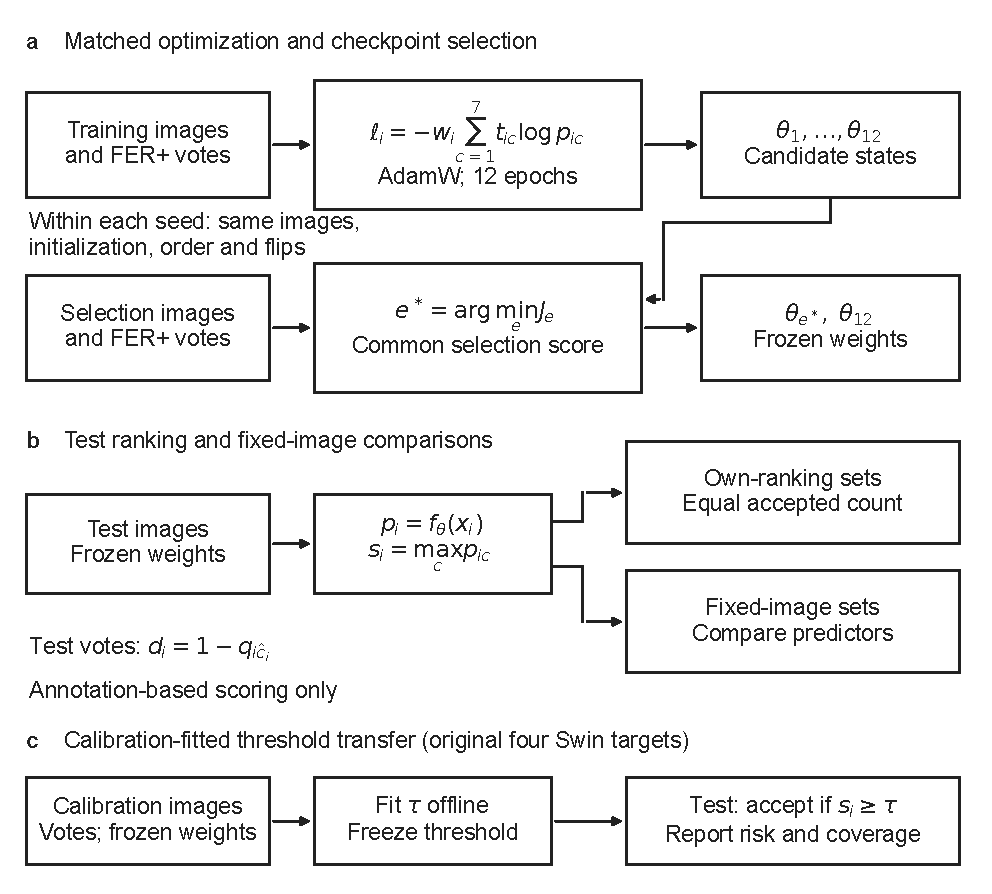
\includegraphics[width=\linewidth]{submission_reader_2026_10_13/source/figures/Fig1.pdf}
\caption{Within-source experimental design. (a) Training uses target $t_i$ and weight $w_i$. Selection minimizes $J_e$, the selection-set ten-category squared distance with $p_e$ padded by three zeros, to choose $\theta_{e^*}$; $\theta_{12}$ is retained independently. (b) Frozen models provide test probabilities and maximum-probability scores. Own-ranking fixes the accepted count; cross-evaluation fixes the images. Test votes only score predictions. (c) Calibration votes fit threshold $\tau$, which stays fixed for testing. Only this branch fits a threshold, and it uses the original four Swin conditions}\label{fig:design}
\end{figure}
\subsection{Matched hard and soft supervision}
Figure~\ref{fig:targets} illustrates the five training targets for a unique maximum and a tied maximum. The examples explain the target construction; they are not experimental observations.
\begin{samepage}
Let $q_{ic}$ be the fraction of annotations for image $i$ assigned to category $c$, normalized over all ten categories. The first seven correspond to the supported expression outputs. Define supported mass $w_i=\sum_{c=1}^{7}q_{ic}$ and $r_{ic}=q_{ic}/w_i$ when $w_i>0$. For model probabilities $p_{ic}$, the two per-image objectives are
\begin{align}
\ell_i^{\mathrm{hard}}&=-w_i\log p_{i h_i},\quad h_i=\arg\max_{c\leq7}r_{ic},\\
\ell_i^{\mathrm{soft}}&=-w_i\sum_{c=1}^{7}r_{ic}\log p_{ic}
                     =-\sum_{c=1}^{7}q_{ic}\log p_{ic}.
\end{align}
All conditions use the same images and weights, with loss averaged over batch size rather than total supported mass. The 152 Training rows with no votes for supported categories contribute zero supervised loss. Among positive-mass rows, 1,360 have tied maximum votes, which Hard resolves using the fixed class order.
\end{samepage}

The controls separate aspects of the target representation that a Hard--Soft comparison changes together. Uniform preserves the largest training-target probability by assigning $m_i=\max_c r_{ic}$ to the dominant class $h_i$ chosen by the fixed class order, and $(1-m_i)/6$ to every other class. Tie-hard instead assigns $1/|T_i|$ to each member of $T_i=\{c:q_{ic}=\max_{k\leq7}q_{ik}\}$ and zero otherwise. Both minimize $-w_i\sum_c t_{ic}\log p_{ic}$. Uniform compares the observed allocation among minority categories with image-dependent uniform softening; unlike constant label smoothing, its dominant probability varies by image. Tie-hard gives the expected loss of uniformly resolving tied maxima without additional random draws, and equals Hard on unique maxima. These conditions keep the images, weights and output vocabulary fixed rather than removing ambiguous images or manually relabeling them.

A third control, Tie-Uniform, preserves every tied maximum. With $k_i=|T_i|$, its target is
\begin{equation}
t_{ic}^{\mathrm{TU}}=\begin{cases}m_i,&c\in T_i,\\(1-k_i m_i)/(7-k_i),&c\notin T_i,\ k_i<7.\end{cases}
\end{equation}
When $k_i=7$, all targets are $1/7$; rows with zero supported mass retain zero loss. Tie-Uniform equals Uniform on unique maxima and preserves every tied maximum otherwise. Like Uniform, it preserves the largest training-target probability but not entropy or aggregate class marginals. The three additional matched runs therefore test a secondary target-representation contrast rather than a uniquely isolated mechanism.

\begin{figure}[tp]
\centering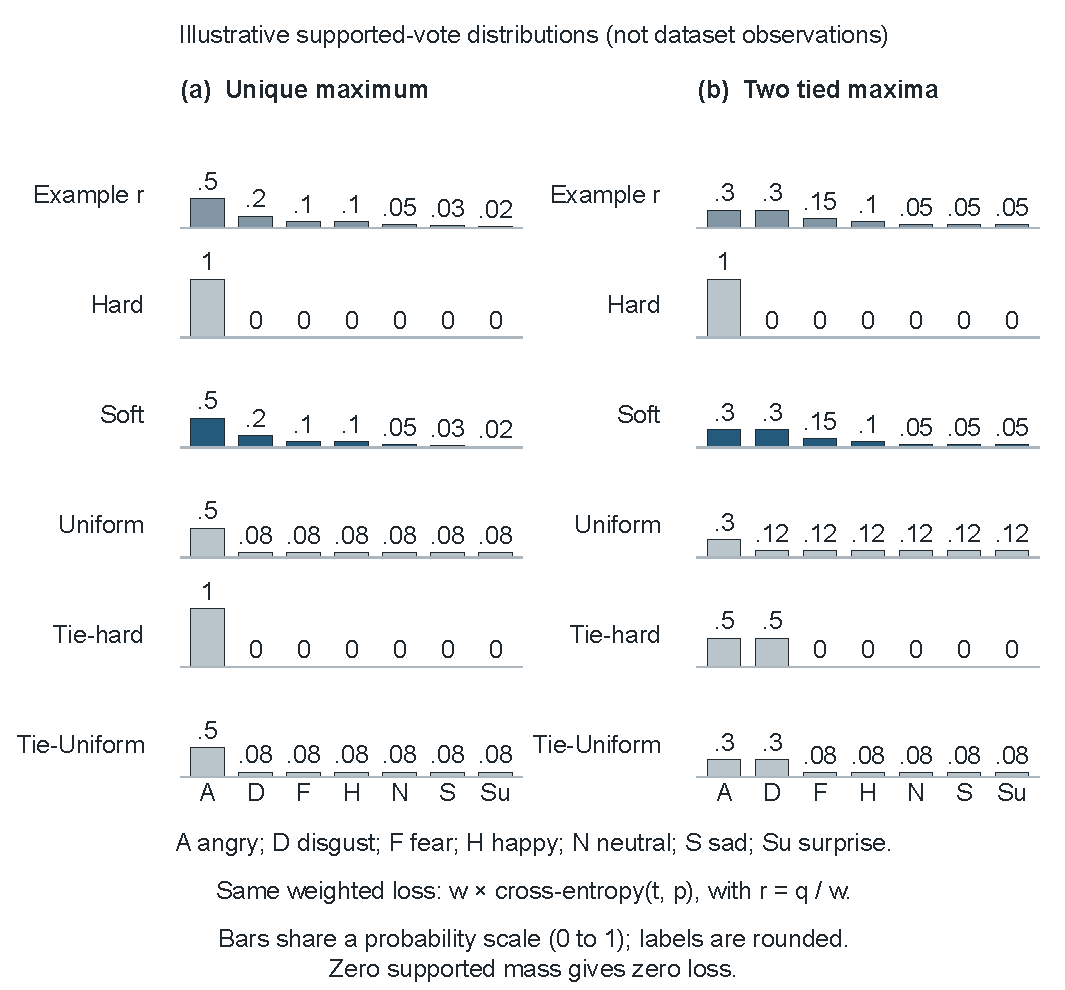
\includegraphics[width=\linewidth]{submission_reader_2026_10_13/source/figures/TargetControls.pdf}
\caption{Illustrative construction of the five training targets from the same supported vote distribution $r$. (a) A unique maximum. (b) Tied maxima. Hard uses the fixed class order to break ties; Tie-hard shares mass across tied maxima. Uniform preserves the chosen maximum probability and spreads the remainder equally. Tie-Uniform preserves every tied maximum and spreads the remaining mass across the other categories. Soft keeps the supported vote distribution. All targets use the same supported-mass weight $w$ in the loss. The examples are constructed for explanation, not selected dataset images}\label{fig:targets}
\end{figure}


\FloatBarrier
\subsection{Architecture, preprocessing, and optimization}
The five Swin-T conditions use torchvision Swin-T with ImageNet-1K V1 initialization \cite{liu2021swin,deng2009imagenet,paszke2019pytorch}. Its pooled feature $z\in\mathbb{R}^{768}$ is gated once, after the backbone:
\begin{equation}
\tilde z=z\odot\sigma\!\left(W_2\operatorname{ReLU}(W_1z)\right),
\quad W_1\in\mathbb{R}^{48\times768},\quad W_2\in\mathbb{R}^{768\times48}.
\end{equation}
The gate layers have no biases, and a linear classifier with bias produces seven logits. The gate adds 73,728 parameters and remains fixed across conditions. Supplementary Fig.~S11 shows the Swin-T hierarchy, feature dimensions and post-pooling head. ResNet-18 uses the same head structure at its own pooled dimension. Because neither backbone is tested without the gate or with another head, these comparisons assess supervision rather than the necessity or superiority of gating.


Images are converted to grayscale, repeated across three channels, resized to $224\times224$ by bilinear interpolation, and normalized with mean and standard deviation 0.5. The fixed output order is angry, disgust, fear, happy, neutral, sad, and surprise. Horizontal flips are the only augmentation and are determined by seed, epoch and original row. For Swin-T, seeds 17, 42, and 89 define three matched groups of five conditions with identical within-seed initialization, sample order, augmentation, architecture and budget. After model construction, the classifier is reset with Torch seed $1000+\mathrm{seed}$. Initial-state hashes and configuration comparisons verify this match.

All backbone and head parameters are optimized for 12 epochs with AdamW \cite{loshchilov2019adamw}, batch size 32, learning rate $10^{-4}$, weight decay $10^{-4}$, and a cosine scheduler with $T_{\max}=12$ and $\eta_{\min}=10^{-6}$, stepped after each epoch. AdamW uses $\beta_1=0.9$, $\beta_2=0.999$, and $\epsilon=10^{-8}$. Training uses BF16 autocast on an NVIDIA RTX 3070 Laptop GPU with 8 GB memory, PyTorch 2.8.0+cu128, and torchvision 0.23.0+cu128. Deterministic algorithms and seeded data loaders control this execution without guaranteeing identical numerical behavior across platforms. The shared budget supports a matched comparison, not a claim of convergence or optimal hyperparameters.

\Needspace{22\baselineskip}
\begin{samepage}
The validation-selected checkpoint minimizes mean squared distance from the complete ten-category vote distribution on the selection subset, after padding the seven predicted probabilities with three zeros; earlier epochs resolve ties. This shared criterion avoids selecting a condition by original-label F1. All five conditions are evaluated at both the selected and fixed epoch-12 checkpoints. The fixed-epoch comparison removes checkpoint selection as a stopping decision, although selection by another metric cannot be reconstructed because not all intermediate weights were retained. Both evaluated sets of weights, logs and probabilities accompany the supplementary package. For fixed annotations, squared distance differs from expected multiclass Brier loss against one annotation draw by $1-\lVert q_i\rVert_2^2$, a model-independent constant, providing a common probability-sensitive objective rather than either categorical reference.

The shared selection criterion nevertheless has a different ideal target from weighted soft cross-entropy. For one image with $w>0$, weighted soft cross-entropy is minimized by $p_c=q_c/w$. Minimizing ten-category squared distance under $\sum_{c\leq7}p_c=1$ instead gives $p_c=q_c+(1-w)/7$ by a Lagrange multiplier. This nonnegative solution sums to one. The targets coincide at $w=1$ but generally differ otherwise, motivating the fixed-epoch and supported-mass diagnostics rather than an assumption that the criterion is neutral between supervision targets.
\end{samepage}

\subsection{Second-backbone robustness check}
The final adaptive phase uses ResNet-18 \cite{he2016resnet} with torchvision ImageNet-1K V1 initialization. Its pooled 512-vector passes through one bias-free $512\!\to\!32\!\to\!512$ ReLU/sigmoid gate (32,768 parameters) and a seven-logit classifier with bias. Soft, Uniform and Tie-Uniform each use seeds 17, 42 and 89, sharing initialization, image order and augmentation within a seed. Data roles, transforms, losses, optimization, budget and selection criterion remain unchanged. BatchNorm follows standard training updates, including training images with zero supported mass, which can affect its statistics despite contributing no direct supervised loss. Retaining the shared transform instead of ResNet's default ImageNet transform keeps preprocessing matched. The differing backbone behavior and gate dimensions make this a secondary supervision-robustness check, not an optimized architecture comparison. All nine runs finish and are hashed before calibration/test inference; reporting includes selected and epoch-12 states, both 80\% contrasts, fixed-image cross-evaluations and vocabulary/reference diagnostics regardless of direction.

\subsection{Disagreement, annotation floor, and classification metrics}
For predicted category $\hat c_i=\arg\max p_i$, expected disagreement with one draw from the observed annotations is $d_i=1-q_{i\hat c_i}$. This quantity measures agreement with the empirical annotations.

For illustration, suppose that six of ten annotations assign an image to happy and four assign it to neutral. Predicting happy gives disagreement 0.4, whereas predicting neutral gives disagreement 0.6. These are constructed values illustrating the definition, not dataset observations. A model may improve its probability estimate of this distribution while retaining happy as its predicted category, leaving category disagreement unchanged. Squared distributional distance evaluates the probability allocation, whereas the disagreement score evaluates the selected category.

The lowest disagreement available to a seven-category predictor is the annotation floor $b_i=1-\max_{c\leq7}q_{ic}$, giving
\begin{equation}
d_i=b_i+e_i,\qquad e_i=\max_{c\leq7}q_{ic}-q_{i\hat c_i}\geq0.
\label{eq:decomposition}
\end{equation}
The floor includes both disagreement among supported categories and votes outside the model's vocabulary. Reporting the mean floor, excess $e_i$ and total disagreement on identical accepted images separates accepted-set composition from category choice relative to the finite observed votes. The secondary measure of probability allocation is
\begin{equation}
D=\frac{1}{N}\sum_{i=1}^{N}\sum_{c=1}^{10}(\tilde p_{ic}-q_{ic})^2,
\end{equation}
where $\tilde p_i=(p_{i1},\ldots,p_{i7},0,0,0)$ and $q_i$ retains all ten vote categories without renormalizing to supported outputs. The distance sums over categories and averages over all $N=3,275$ primary test images for every available target, seed and selected/epoch-12 state. It measures test-set distributional agreement, distinct from the selection-set objective and confidence-selected category disagreement; a lower value alone does not establish calibration.

The disagreement further decomposes algebraically into unsupported vote mass, supported-category ambiguity and excess disagreement:
\begin{equation}
d_i=\underbrace{1-w_i}_{\text{unsupported mass}}+
\underbrace{w_i-\max_{c\leq7}q_{ic}}_{\text{supported ambiguity}}+e_i.
\label{eq:threeparts}
\end{equation}
For an ideal model with $p_i=r_i$, disagreement is $1-w_i\max_c p_{ic}$. Maximum softmax probability (MSP) omits $w_i$: an MSP of 0.9 implies disagreement 0.1 when $w_i=1$, but 0.55 when $w_i=0.5$. This hypothetical example illustrates how supported mass enters the reference definition, without attributing the observed transfer failure solely to omitted mass. Annotation-derived $w_i$ is unavailable for a new runtime image and is not used as a deployment selector.

Results are stratified by $w=0$, $0<w<1$, and $w=1$. Restricting a model's global 80\% accepted set to each stratum differs from selecting 80\% separately within each stratum; both analyses are labeled. For positive-mass images, supported-only disagreement, $1-r_{i\hat c_i}$, provides an additional conditional endpoint. Because it changes the reference population of votes, it complements rather than replaces complete-vote risk or an expanded-vocabulary model experiment.

Secondary classification metrics use explicit categorical references \cite{sokolova2009metrics}. Against the original FER2013 labels, weighted F1 is $\sum_c n_c F1_c/N$ and macro F1 averages the seven $F1_c$ values equally, assigning zero to undefined class scores. Crowd-majority weighted F1 instead includes only images with more than half of all votes assigned to one supported category, with its denominator reported. These references define different tasks, so their F1 values are not compared as interchangeable scores. Full-vote outcomes retain images without a majority.

\subsection{Selection, calibration, and uncertainty}
The primary follow-up endpoint is the Soft-minus-Uniform difference in mean vote disagreement at 80\% common test coverage. The original Soft-minus-Hard contrast is retained, while Tie-hard and fixed-epoch contrasts provide sensitivity analyses. Each fitted model ranks images by MSP and accepts exactly $\lceil0.8N\rceil$, resolving score ties by original row order. Equal counts allow a common-coverage ranking comparison but do not ensure identical accepted images. No deployment threshold is fitted on test labels. Coverage values 20\%, 50\%, and 100\% and all-prefix curves provide secondary descriptions.

Calibration transfer instead fits thresholds on the separate calibration subset, maximizing accepted count subject to empirical mean vote disagreement no greater than 10\%, 20\%, or 30\%. Each qualifying threshold must accept at least 100 calibration images without splitting score ties; if none qualifies, the policy abstains completely. The threshold is then frozen and applied unchanged to the primary test population. These empirical targets provide operating points, not confidence-bound guarantees, and test risk may exceed the target.

For a conservative comparator, thresholds lie on a fixed 101-point grid from zero to one. At each threshold retaining $n\geq100$ calibration rows, define
\begin{equation}
U=\min\!\left\{1,\bar d+\sqrt{\frac{\log(101/0.05)}{2n}}\right\}.
\end{equation}
The comparator maximizes coverage subject to $U$ not exceeding the target, otherwise abstaining completely. Hoeffding's inequality \cite{hoeffding1963} and a union bound give simultaneous per-model control over the fixed grid for bounded, independent and identically distributed losses, a fixed fitted model and an unchanged population. Our reused, potentially dependent images and an unverified deployment population do not justify that guarantee. The comparator therefore illustrates the coverage cost of an established finite-sample margin; empty accepted sets have undefined risk rather than zero error.

At each empirical operating point, the calibration-to-test change in mean risk is partitioned into the three terms of Eq.~\ref{eq:threeparts}, using each population's accepted set. Full-population summaries provide context for these conditional comparisons. To examine within-calibration variation, 100 deterministic pixel-cluster half-splits fit each empirical threshold on one half and evaluate it on the disjoint half, with assignments shared across models. The overlapping resamples describe search optimism and sample variation rather than independent replications or a causal explanation of the test-risk overshoot.

Each within-backbone contrast is reported for all three paired seeds. A 5,000-replicate paired exact-pixel-cluster bootstrap shares sampled cluster multiplicities across compared models and reranks each replicate at 80\% coverage. Percentile intervals describe sensitivity to sampled images conditional on the fitted models, seeds and observed annotations; they exclude person-level dependence, annotation uncertainty, seed-population variability and prior hypothesis selection. Soft-minus-Tie-Uniform is a prespecified secondary contrast in the final adaptive phase. The validation-selected Swin-T Soft-minus-Uniform comparison remains the only primary follow-up contrast, with ResNet comparisons serving as adaptive secondary robustness checks. Other intervals describe sensitivities without multiple-comparison significance claims, and a zero-crossing interval does not establish equivalence.


\subsection{Exploratory confidence-score sensitivity}
The exploratory score analysis compares three functionals fixed before their additional comparative summaries were computed: MSP, the top-two margin $p_{(1)}-p_{(2)}$, and negative entropy $\sum_{c=1}^{7}p_c\log p_c$, where $p_{(1)}\geq p_{(2)}$ and $0\log0=0$. All rank the same frozen probabilities, increase with confidence, and leave predicted categories and crowd annotations unchanged. Original row ID resolves exact ties, and each score accepts $\lceil\gamma N\rceil$ images at coverage $\gamma\in\{0.2,0.5,0.8,1.0\}$. The ledger includes all 48 states and every available target, with both controls, backbone families and checkpoint states reported at 80\% coverage. These are own-ranking comparisons, not identical-image or threshold-transfer experiments. Paired-seed differences are descriptive, without new intervals or significance claims. The exploratory status follows from the previously examined MSP and test outcomes described in the study design; neither calibration-transfer policies nor the prototype are changed.


\subsection{Frozen-checkpoint external clip evaluation}\label{sec:external}
RAVDESS supplies original human category judgments for external evaluation \cite{livingstone2018ravdess}. We use all 1,440 video-only speech clips from 24 actors, with ten responses per clip and no audio. The unmodified S5 workbook provides nine response options: the seven model categories, calm, and none. The professional actors were aged 21--33 and recruited in Toronto, defining a limited acted-video population rather than a naturalistic messaging sample. Media were obtained from the original Zenodo record under CC BY-NC-SA 4.0 and are not redistributed; Online Resource 8 records archive and clip integrity checks. Changes in recording conditions, actor population and judgment unit make this an external clip-transfer test rather than a static-image benchmark replication. Figure~\ref{fig:externalpipeline} separates frozen prediction from annotation-based scoring.

All 36 existing Soft, Uniform and Tie-Uniform states (two families, three seeds, selected and epoch 12) are evaluated without external fitting, checkpoint choice, threshold fitting or expression-peak selection. Hard and Tie-hard are outside this contrast family. The protocol samples eight bin centers $\lfloor(b+0.5)N/8\rfloor$, $b=0,\ldots,7$, from a clip of $N\geq8$ frames. Each frame requires exactly one MediaPipe detection (model selection 1, minimum confidence 0.5) and a valid crop from the shared routine, clipped to image bounds. Boxes are not expanded, and neither fallback detectors nor manual crop repairs are used. The original grayscale-three-channel, bilinear $224\times224$, mean/std 0.5 transform is retained. A clip requires at least four valid distinct frames to receive a prediction.

Inference uses the earlier benchmark's CUDA BF16 forward pass and float32 softmax. The arithmetic mean of valid-frame probabilities, computed in float64, defines clip probabilities before argmax. This fixed aggregation is neither a temporal model nor the prototype's FP32 single-frame update rule. Frame probabilities, clip means, crop diagnostics and failures are retained. All 1,440 clips remain in the coverage denominator. At coverage $\gamma$, MSP accepts the top $\lceil\gamma\,1440\rceil$ eligible clips, resolving ties by filename order. An endpoint is unavailable if eligibility is insufficient; unavailable values are not imputed. Risk across all eligible clips and maximum achievable coverage are reported separately, with margin, negative entropy and coverages 20\%, 50\% and 100\% as prespecified sensitivities.

Complete-reference disagreement is $1-q_{i\hat c_i}$, with the same three-term accounting as Eq.~\ref{eq:threeparts}. The primary reference retains all nine responses. A required sensitivity analysis merges calm into neutral while leaving none unchanged, following the original study's neutral/calm interchangeability convention without editing raw counts. These endpoints compare predictions with human response distributions rather than intended-expression labels or published RAVDESS accuracy. Soft-minus-Uniform at 80\% MSP for validation-selected Swin-T is the principal contrast. Reporting includes both controls, families and checkpoint states, all three paired seeds, and 80\% MSP fixed-image cross-evaluations regardless of direction.

\begin{figure}[tp]
\centering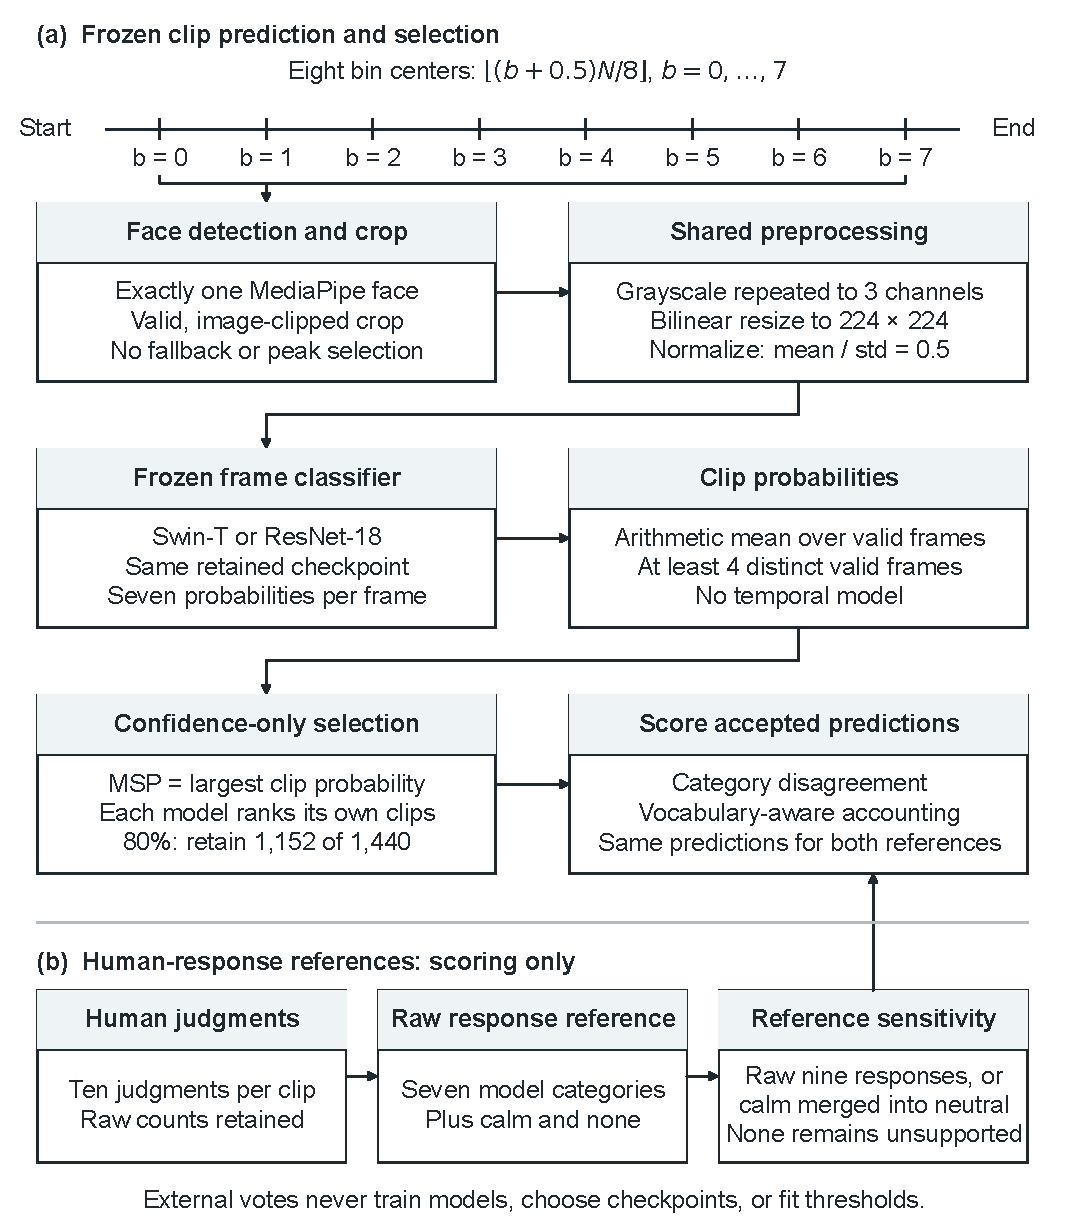
\includegraphics[width=\linewidth]{submission_reader_2026_10_13/source/figures/ExternalPipeline.pdf}
\caption{Frozen-model transfer from static-image training to external video clips. Eight bin-center frames are sampled without selecting expression peaks. Valid single-face crops undergo the shared preprocessing and frozen-model inference; valid-frame probabilities are averaged before clip prediction and confidence ranking. At least four valid distinct frames are required, and every clip remains in the coverage denominator. Human responses enter scoring only. The raw reference retains nine responses; the sensitivity reference adds calm to neutral and retains none, without changing predictions or accepted clips. No external optimization, threshold fitting or temporal model is used}\label{fig:externalpipeline}
\end{figure}

External uncertainty is summarized by 5,000 paired actor-cluster bootstrap samples, resampling 24 whole actors with replacement (RNG seed 11011). Each replicate contains 1,440 clips because each actor contributes 60, and is reranked at 80\% of the repeated clip multiset. Shared actor multiplicities preserve pairing across seeds, conditions and references. Percentile 95\% intervals summarize mean paired-seed contrasts for both controls, families and checkpoint states; any replicates with insufficient eligibility are disclosed and preclude a complete interval. These intervals condition on the fitted models, observed actors and votes rather than unrestricted seed, rater or demographic populations, and are not used for multiple-testing superiority claims. Before outcome interpretation, source-overlap screening compares canonical $48\times48$ grayscale crop hashes and 63-bit AC DCT perceptual hashes with all 35,887 FER2013 images. Hamming distance at most four is a review flag, not an automatic exclusion or proof of identity overlap; an absent match does not establish person-disjointness. Online Resource 8 retains complete outputs and independent recomputation alongside the protocol and integrity records.

\subsection{Post hoc retained-output diagnostics}
The post hoc diagnostics summarize external category counts across all eligible clips and at the original 80\% MSP endpoint for every condition, checkpoint state and seed. Their exploratory status and timing are specified in the study design. For accepted clip set $A$, reference category $a$ and predicted category $b$, the vote-weighted matrix is
\begin{equation}
C_{ab}(A)=\sum_{i\in A}q_{ia}\,\mathbb{I}(\hat c_i=b).
\end{equation}
Row normalization divides by $\sum_{i\in A}q_{ia}$ and is undefined when that mass is zero. Rows for unsupported reference categories remain in the display. Because entries are fractional annotation contributions, they are not independent participant observations or ordinary single-label confusion counts. Raw and merged references score unchanged predictions and accepted IDs.

Temporal summaries report mean neutral probability, category frequencies and frame-to-aggregate-clip argmax agreement across all eight bins, using valid-frame denominators. Human judgments apply to clips, so these are prediction diagnostics rather than frame-accuracy measures. Acquisition and response mapping, frame indices and crops, checkpoint identities, probability normalization and exact mean-probability aggregation are verified before interpretation. The diagnostics introduce no peak selection, filtering, fitting or new inferential test.

\subsection{Implementation and verification boundary}
The sender-controlled local prototype uses MediaPipe detection \cite{lugaresi2019mediapipe} with the shared image transform, class order and Swin model head, suppressing invalid, stale or unapproved cues. ResNet remains a research robustness check rather than an application model. Online Resource 1 documents the prototype's runtime, local-processing and transmission boundaries, unvalidated sender controls and absence of demonstrated communication benefit. The application is an implementation artifact, not the empirical validation setting. Code checks cover numerical metrics, checkpoint requirements and failure states. AI assistance (OpenAI Codex) was used for literature checking, experimental and analysis code, manuscript drafting, and technical verification; the authors remain responsible for methods, results, source accuracy and final submission.

\FloatBarrier
\Needspace{8\baselineskip}
\section{Results}
% Editorial Results entry point: the order follows the scientific questions.
\subsection{Effects of supervision targets and checkpoint selection}
The primary comparison concerns whether the supported-category vote distribution improves selective predictions beyond preserving the dominant target probability. At 80\% coverage, validation-selected Swin-T models trained with Soft have mean complete-vote disagreement of 23.68\%, compared with 24.06\% for Uniform (Table~\ref{tab:primary}). The paired Soft-minus-Uniform difference is -0.38 pp, with a conditional 95\% interval of [-0.64, -0.07]. This is a modest advantage over the matched softening control; each model selects its own accepted images.
\begin{table}[t]
\caption{Selected-checkpoint risk at 80\% coverage (2,620 of 3,275 images). Risk is mean $\pm$ sample SD; components are mean percentage points}\label{tab:primary}
\centering\begin{tabular}{lrrrr}\toprule
Targets & Risk (\%) & Unsupported & Ambiguity & Excess\\\midrule
Hard & $26.30 \pm 1.04$ & 6.65 & 16.14 & 3.51\\
Tie-hard & $25.82 \pm 0.58$ & 6.67 & 16.03 & 3.13\\
Uniform & $24.06 \pm 0.10$ & 6.41 & 15.41 & 2.24\\
Tie-Uniform & $24.27 \pm 0.17$ & 6.47 & 15.46 & 2.35\\
Soft & $23.68 \pm 0.07$ & 6.55 & 15.01 & 2.13\\
\bottomrule\end{tabular}\par
Accepted identities differ; components provide accounting, not causal attribution.
\end{table}


The retained comparisons with hard targets show why the control matters. Soft minus Hard is -2.61 pp (conditional 95\% interval [-2.98, -2.19]), substantially larger than the primary Soft-minus-Uniform contrast. Tie-hard minus Hard is -0.47 pp (interval [-0.80, -0.12]), while Soft minus Tie-hard is -2.14 pp (interval [-2.49, -1.76]). These secondary intervals describe sensitivity to the target construction, rather than additional primary hypothesis tests.

The direction of the primary Swin-T contrast persists when the checkpoint is retained after 12 epochs instead of selected by validation distance. Soft minus Uniform is then -0.32 pp (conditional 95\% interval [-0.63, -0.05]); Soft minus Hard is -1.35 pp (interval [-1.72, -1.05]). Table~\ref{tab:sensitivity} reports the absolute risks at both checkpoint states. This comparison changes checkpoint selection, not the training budget or objective.
\begin{table}[t]
\caption{Selected versus fixed epoch-12 complete-vote risk at 80\% coverage (\%); means across three paired seeds}\label{tab:sensitivity}
\centering\begin{tabular}{lrr}\toprule
Targets & Selected & Epoch 12\\\midrule
Hard & 26.295 & 24.983\\
Tie-hard & 25.824 & 24.576\\
Uniform & 24.062 & 23.949\\
Tie-Uniform & 24.272 & 23.939\\
Soft & 23.684 & 23.632\\
\bottomrule\end{tabular}\par

\end{table}


The tie-preserving control gives the same qualitative result for Swin-T. Soft has lower disagreement than Tie-Uniform at both checkpoint states, with conditional intervals below zero (Table~\ref{tab:backbones}). Unlike Uniform, Tie-Uniform does not favor a single category when the highest vote counts are tied. Both controls nevertheless differ from Soft in entropy and aggregate class proportions, so these comparisons do not isolate the effect of minority-category identity alone. The supplementary learning and selection curves retain all training trajectories; loss magnitudes across different target constructions are not directly comparable measures of fitting quality.

Figure~\ref{fig:difference} places the primary endpoint in the broader coverage range. It is a descriptive comparison using each model's own confidence ranking, not an additional confirmatory test.
\begin{figure}[tp]\centering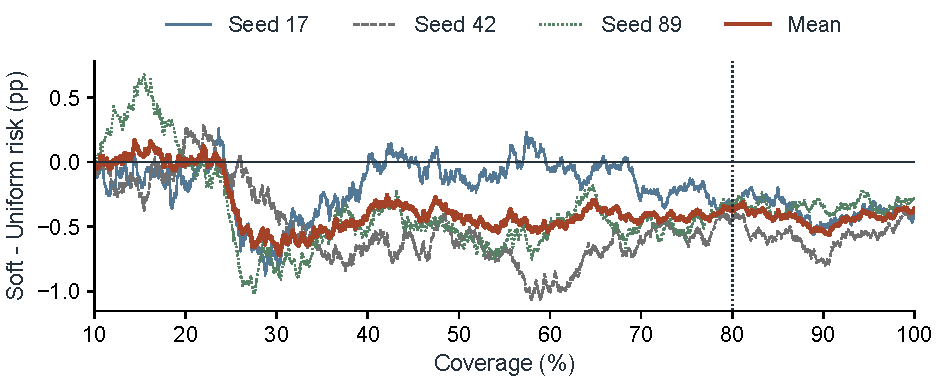
\includegraphics[width=\linewidth]{submission_reader_2026_10_13/source/figures/Fig5.pdf}
\caption{Soft-minus-Uniform complete-vote disagreement versus common coverage. Thin curves show paired seeds; the thick curve shows their mean. Each model uses its own ranking, rather than an identical accepted-image set. The vertical marker identifies the primary 80\% endpoint. No simultaneous uncertainty band is estimated}\label{fig:difference}\end{figure}

\subsection{Distributional agreement and backbone sensitivity}\label{sec:distance}

The secondary distributional endpoint gives a more consistent result than selective category disagreement. Soft has lower squared distance than both controls in every tested seed, backbone and checkpoint state (Table~\ref{tab:distance}). For validation-selected Swin-T, mean distance is 0.09783 for Soft and 0.11571 for Uniform. This endpoint evaluates the complete probability vector on all 3,275 primary-test images, without confidence rejection. Supplementary Sect.~S2 provides the per-seed values for all five Swin-T and three ResNet-18 targets.

\begin{table}[t]\caption{Agreement with the complete crowd-vote distribution. Ten-category squared distances are averaged across three separate seeds on the same 3,275 test images. Lower is better; values are unscaled distance units, not percentages}\label{tab:distance}

\centering\small\begin{tabular}{llrrrrr}\toprule

Backbone & State & Soft & Uniform & Tie-Uniform & $\Delta_U$ & $\Delta_{TU}$\\\midrule

Swin-T & Selected & 0.09783 & 0.11571 & 0.11373 & -0.01787 & -0.01589\\

Swin-T & Epoch 12 & 0.09779 & 0.11699 & 0.11280 & -0.01920 & -0.01501\\

ResNet-18 & Selected & 0.11059 & 0.12303 & 0.11805 & -0.01244 & -0.00746\\

ResNet-18 & Epoch 12 & 0.11089 & 0.12259 & 0.11665 & -0.01170 & -0.00576\\

\bottomrule\end{tabular}\par\smallskip

$\Delta_U$ and $\Delta_{TU}$ are Soft minus Uniform and Soft minus Tie-Uniform. For each image, the score sums ten squared probability differences after adding three zero entries to the seven model outputs. It then averages across images. Vote distributions are not renormalized to the supported categories. Model probabilities are not combined across seeds.\par\end{table}

The adaptive ResNet-18 checks distinguish this distributional advantage from the selective result. For validation-selected ResNet-18, Soft-minus-Uniform disagreement is +0.173 pp, compared with -0.378 pp for Swin-T. All four ResNet-18 conditional intervals cross zero (Table~\ref{tab:backbones}), so these checks do not confirm Swin-T's selective advantage. Supplementary Sect.~S2 reports the per-seed contrasts and accompanying diagnostics. These are architecture-sensitivity checks using the same source images and adaptive study design, not independent-image confirmation.
\begin{table}[t]
\caption{Within-backbone Soft-minus-control disagreement at 80\% coverage (percentage points). Intervals condition on fitted models, three seeds, observed pixels and votes}\label{tab:backbones}
\centering\begin{tabular}{lllrr}\toprule
Backbone & State & Control & Difference & 95\% interval\\\midrule
Swin-T & selected & Uniform & -0.378 & [-0.644, -0.073]\\
Swin-T & selected & Tie-Uniform & -0.588 & [-0.830, -0.281]\\
Swin-T & epoch12 & Uniform & -0.317 & [-0.626, -0.050]\\
Swin-T & epoch12 & Tie-Uniform & -0.307 & [-0.585, -0.024]\\
ResNet-18 & selected & Uniform & +0.173 & [-0.167, +0.455]\\
ResNet-18 & selected & Tie-Uniform & +0.042 & [-0.258, +0.343]\\
ResNet-18 & epoch12 & Uniform & +0.170 & [-0.157, +0.467]\\
ResNet-18 & epoch12 & Tie-Uniform & +0.190 & [-0.126, +0.515]\\
\bottomrule\end{tabular}\par
\smallskip
ResNet comparisons are adaptive secondary robustness checks, not independent-image confirmation or architecture comparisons.\par
\end{table}


Figure~\ref{fig:backbones} brings the two endpoints together. Squared distance measures agreement across the complete annotation distribution, whereas category disagreement depends on the predicted category and, under confidence selection, the accepted-image set. Better distributional agreement can therefore coexist with little or no selective category advantage. The result concerns the tested source-dataset configurations; it does not establish deployment calibration or better external transfer.
\begin{figure}[tp]\centering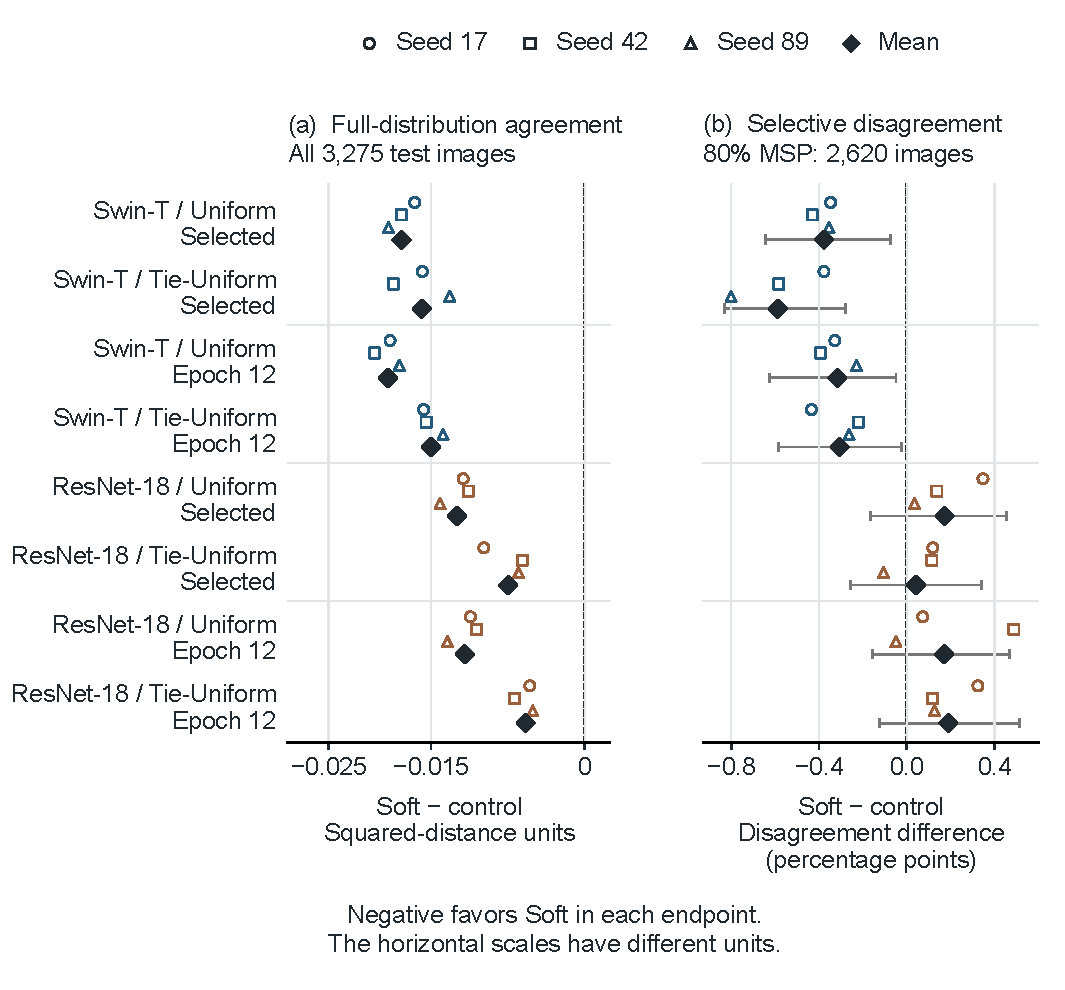
\includegraphics[width=\linewidth]{submission_reader_2026_10_13/source/figures/Fig7.pdf}
\caption{Distributional agreement and selective disagreement for Soft relative to the matched controls. (a) Ten-category squared-distance differences on all 3,275 primary-test images, in unscaled distance units. (b) Complete-vote disagreement differences at 80\% coverage using each model's ranking, in percentage points. Symbols show the three paired-seed contrasts and their mean. Bars in (b) are 95\% pixel-cluster bootstrap intervals conditional on the fitted models and observed votes; no interval is shown in (a). Both backbones and validation-selected and epoch-12 checkpoints are included. Negative values favor Soft. The panels use different units and scales}\label{fig:backbones}\end{figure}


\subsection{Accepted-image sets and annotation references}
For validation-selected Swin-T, the predictor comparison depends on the accepted-image set. Soft-minus-Uniform disagreement is +0.085 pp on images selected by Uniform, but -0.352 pp on images selected by Soft (Fig.~\ref{fig:cross}). Each within-column comparison holds the images and annotation reference fixed, so the difference reflects the predictors' category choices on that set. Lower risk under Soft's own ranking therefore does not establish consistently better category predictions on identical images.
\begin{figure}[tp]\centering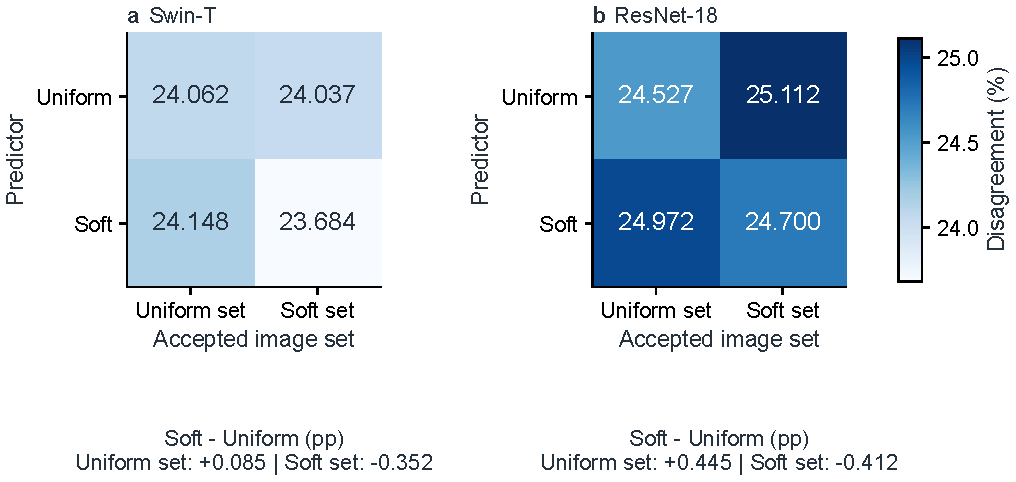
\includegraphics[width=\linewidth]{submission_reader_2026_10_13/source/figures/Fig4.pdf}
\caption{Fixed-image cross-evaluation at 80\% coverage for validation-selected (a) Swin-T and (b) ResNet-18 checkpoints. Cells are complete-vote disagreement percentages averaged across three seeds. Columns fix the selector's 2,620-image set; rows change the predictor. The common color scale shows absolute risk, and signed differences below each panel show within-column Soft-minus-Uniform contrasts. Each model's own-set risk uses a different accepted set}\label{fig:cross}\end{figure}

Changing the accepted set also changes the result for a fixed predictor. Moving from Uniform-selected to Soft-selected images gives a risk change of -0.025 pp for the Uniform predictor and -0.463 pp for the Soft predictor. The mean Jaccard overlap is 0.8408. The ResNet-18 Soft-minus-Uniform comparison likewise changes sign between Uniform-selected (+0.445 pp) and Soft-selected images (-0.412 pp). These patterns show an interaction between prediction and selection rather than a unique causal contribution from either. The supplement retains every seed, both checkpoint states, the complete cross-evaluation matrices and overlap counts.

Changing the annotation reference altered the measured classification performance without changing the predictions. On the same 2,484 supported-majority images, validation-selected Swin-T models trained with Soft had mean weighted F1 of 0.6685 against the original FER2013 labels and 0.9270 against the crowd-majority labels (Table~\ref{tab:samef1}). Image selection also affected the score: under the original FER2013 reference, weighted F1 increased from 0.5722 on all 3,275 primary-test images to 0.6685 on this subset. The first comparison changes the label reference while holding images fixed; the second changes the image population while retaining the original reference. The crowd-majority score therefore describes a different evaluation task from original-label performance on the complete test population, not an improvement in the underlying predictions. The supplementary reference matrix documents the correspondence between the two categorical references. Neither reference is treated as a measure of internal emotion.
\begin{table}[t]
\caption{Weighted F1 under two label references for selected models: means across three seeds}\label{tab:samef1}
\centering\begin{tabular}{lrrr}\toprule
Targets & Original/all & Original/subset & Crowd/subset\\\midrule
Hard & 0.5658 & 0.6580 & 0.8965\\
Tie-hard & 0.5599 & 0.6572 & 0.9032\\
Uniform & 0.5683 & 0.6642 & 0.9205\\
Tie-Uniform & 0.5662 & 0.6619 & 0.9195\\
Soft & 0.5722 & 0.6685 & 0.9270\\
\bottomrule\end{tabular}\par
All: 3,275 images; subset: the same 2,484 supported-majority images in the last two columns. No retraining or relabeling is performed.
\end{table}


\subsection{Effects of unsupported annotation categories}
The primary-test population includes 1,732 fully supported images, 1,527 with both supported and unsupported vote mass, and 16 with zero supported mass. Figure~\ref{fig:mass} separates unsupported mass, supported-category ambiguity and excess disagreement on each global accepted set, then compares confidence rankings within the supported-mass strata. At 80\% within-stratum coverage, Soft and Uniform have disagreement of 10.42\% and 10.94\% in the fully supported stratum, and 40.00\% and 40.58\% in the partially supported stratum. The primary contrast is thus not confined to images receiving unsupported votes. These descriptive strata do not explain the confidence assigned to individual images.
\begin{figure}[tp]
\centering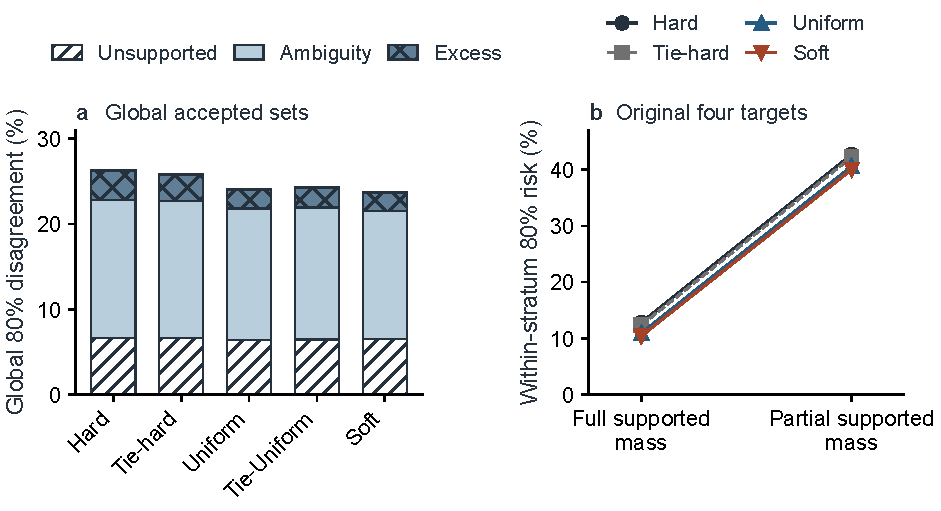
\includegraphics[width=\linewidth]{submission_reader_2026_10_13/source/figures/Fig3.pdf}
\caption{Risk components at 80\% coverage. (a) All five Swin-T targets on each model's global accepted set. (b) The original four targets with selection performed separately within the full- and partial-supported-mass strata. Panels use different populations and vertical scales. Zero-supported-mass images have complete-vote disagreement one; their acceptance counts appear in Table~\ref{tab:retention}. Unsupported votes remain in every score}\label{fig:mass}
\end{figure}

Overall risk also conceals differences in which unsupported images are accepted. Soft accepts a mean 11.00 of the 16 zero-supported-mass images, compared with 7.00 for Uniform and 6.67 for Tie-Uniform (Table~\ref{tab:retention}). Its lower overall disagreement therefore does not imply more effective rejection of these images. The counts are small and descriptive, rather than estimates of a deployment failure rate. The supplement reports contempt, unknown and not-a-face vote mass separately because these categories have different meanings, including all-image and accepted-set summaries for calibration and testing.
\begin{table}[t]
\caption{Accepted image counts at global 80\% coverage, seeds 17, 42, 89 in that order. Population sizes: full 1,732; partial 1,527; zero 16}\label{tab:retention}
\centering\begin{tabular}{lrrr}\toprule
Targets & Full mass & Partial mass & Zero mass\\\midrule
Hard & 1499, 1501, 1492 & 1115, 1112, 1122 & 6, 7, 6\\
Tie-hard & 1519, 1494, 1508 & 1092, 1119, 1106 & 9, 7, 6\\
Uniform & 1515, 1527, 1527 & 1098, 1087, 1085 & 7, 6, 8\\
Tie-Uniform & 1529, 1522, 1520 & 1084, 1090, 1095 & 7, 8, 5\\
Soft & 1527, 1527, 1533 & 1081, 1083, 1076 & 12, 10, 11\\
\bottomrule\end{tabular}\par
Each seed retains 2,620 images in total. Zero-mass images have disagreement one under every supported prediction.
\end{table}


\subsection{Sensitivity to confidence scores}
\begin{table}[t]
\caption{Exploratory score sensitivity at 80\% coverage: paired-seed mean Soft-minus-control disagreement (pp). Negative values favor Soft; accepted image sets can differ}\label{tab:scores}
\centering\begin{tabular}{lllrr}\toprule
Backbone & State & Score & Uniform & Tie-Uniform\\\midrule
Swin-T & Selected & MSP & -0.378 & -0.588\\
Swin-T & Selected & Margin & -0.153 & -0.299\\
Swin-T & Selected & Neg. entropy & -0.093 & -0.323\\
Swin-T & Epoch 12 & MSP & -0.317 & -0.307\\
Swin-T & Epoch 12 & Margin & -0.122 & -0.057\\
Swin-T & Epoch 12 & Neg. entropy & -0.296 & -0.242\\
ResNet-18 & Selected & MSP & +0.173 & +0.042\\
ResNet-18 & Selected & Margin & +0.417 & +0.206\\
ResNet-18 & Selected & Neg. entropy & +0.509 & +0.485\\
ResNet-18 & Epoch 12 & MSP & +0.170 & +0.190\\
ResNet-18 & Epoch 12 & Margin & +0.511 & +0.555\\
ResNet-18 & Epoch 12 & Neg. entropy & +0.307 & +0.435\\
\bottomrule\end{tabular}\par
\smallskip
MSP reproduces the original ledger exactly. Margin and negative entropy are post hoc sensitivity analyses, not proposed rejection methods. Per-seed results are in Table~S14 and Fig.~S7.\par
\end{table}
The exploratory score analysis retains the mean direction of the backbone-specific comparison at 80\% coverage, but not its magnitude (Table~\ref{tab:scores}). Validation-selected Swin-T favors Soft under MSP, margin and negative entropy, while the corresponding ResNet-18 means favor Uniform. Some individual Swin-T seed contrasts under margin or entropy nevertheless favor Uniform; the supplementary per-seed table shows these reversals. Thus, the average direction at this endpoint is not solely a consequence of using MSP, but neither the score nor the supervision target has a uniform advantage across configurations. At full coverage the three scores give identical risk, since they no longer change the accepted set. These probability-only checks do not compare learned rejection methods.


\subsection{Calibration-to-test transfer}
Empirical thresholds do not preserve their nominal risk targets when transferred unchanged from calibration to testing. Across the original four conditions, all 36 nonempty empirical test settings exceed their targets (Table~\ref{tab:policies}). These settings overlap and are not independent Bernoulli trials. At the 10\% target, Soft attains greater mean coverage than Hard (49.54\% versus 38.35\%), but also greater achieved risk (13.01\% versus 11.45\%). The coverage difference is therefore not a comparison at equal risk.
\begin{table}[t]
\caption{Calibration-fitted policies applied unchanged to primary testing. Entries are mean coverage / risk (\%); coverage includes empty seeds, risk averages nonempty seeds}\label{tab:policies}
\centering\begin{tabular}{llcc}\toprule
Risk target & Supervision & Empirical & Fixed-grid bound\\\midrule
10\% & Hard & 38.35 / 11.45 (3/3) & 0.00 / -- (0/3)\\
10\% & Tie-hard & 39.17 / 11.93 (3/3) & 0.00 / -- (0/3)\\
10\% & Uniform & 45.99 / 12.22 (3/3) & 0.00 / -- (0/3)\\
10\% & Soft & 49.54 / 13.01 (3/3) & 0.00 / -- (0/3)\\
\addlinespace
20\% & Hard & 68.58 / 22.28 (3/3) & 47.03 / 14.55 (3/3)\\
20\% & Tie-hard & 71.04 / 22.80 (3/3) & 48.05 / 14.61 (3/3)\\
20\% & Uniform & 76.20 / 22.80 (3/3) & 57.49 / 16.11 (3/3)\\
20\% & Soft & 76.88 / 22.56 (3/3) & 60.39 / 16.60 (3/3)\\
\addlinespace
30\% & Hard & 98.06 / 32.39 (3/3) & 82.01 / 26.92 (3/3)\\
30\% & Tie-hard & 99.47 / 32.37 (3/3) & 85.41 / 27.54 (3/3)\\
30\% & Uniform & 99.94 / 31.46 (3/3) & 88.41 / 27.11 (3/3)\\
30\% & Soft & 99.91 / 31.07 (3/3) & 89.57 / 27.01 (3/3)\\
\bottomrule\end{tabular}\par
\smallskip\par\footnotesize Parentheses give nonempty test seeds. An empty policy has undefined risk. Neither a nominal target nor the bound's unverified independence/unchanged-population assumptions establish a deployment guarantee. Different achieved risks are not an equal-risk coverage comparison.
\end{table}


The calibration and test populations differ even before confidence selection. Their annotation floors are 23.70\% and 26.67\%, respectively, a +2.97 pp difference; unsupported mass rises from 5.72\% to 7.88\%, with the remainder due to supported-category ambiguity. Figure~\ref{fig:transfer} applies the same accounting to the accepted sets. For Soft at the nominal 20\% target, the +2.57 pp test-minus-calibration risk gap comprises +1.98 pp unsupported mass, +0.78 pp supported ambiguity and -0.19 pp excess. These components describe the gap rather than independent causes.
\begin{figure}[tp]
\centering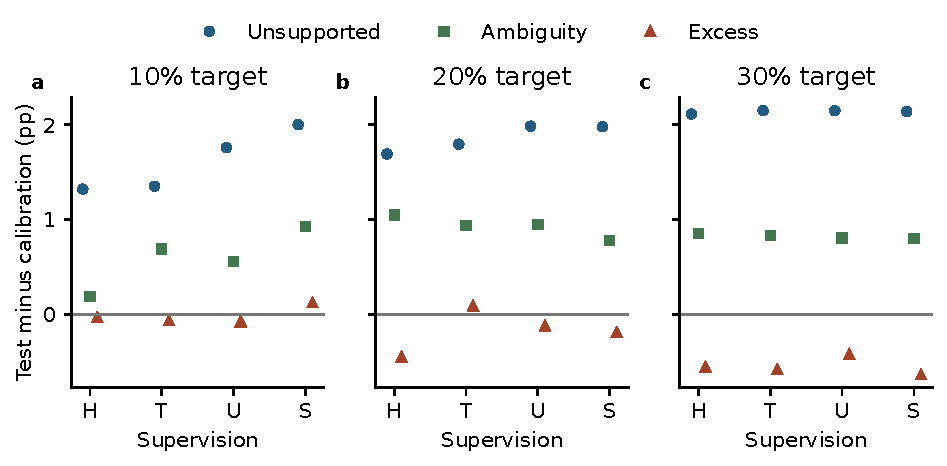
\includegraphics[width=\linewidth]{submission_reader_2026_10_13/source/figures/Fig6.pdf}
\caption{Mean test-minus-calibration differences in unsupported mass, supported ambiguity and excess disagreement for empirical thresholds. Components sum to the risk gap. H: Hard; T: Tie-hard; U: Uniform; S: Soft. The three risk-target panels share a vertical scale. Means use paired nonempty calibration/test accepted sets}\label{fig:transfer}
\end{figure}

The additional diagnostics distinguish variability within calibration from the coverage cost of a more conservative rule. At the 20\% target, calibration-half-split holdout-minus-fit gaps average +0.05 to +0.19 pp across conditions, with broad descriptive 5th--95th-percentile ranges of roughly -2.3 to +2.8 pp. The supplement retains complete per-condition resamples. These summaries do not uniquely separate distribution shift, finite-sample fluctuation and threshold-search effects. The fixed-grid comparator yields 24 nonempty test settings, with 0 exceeding their nominal targets, but rejects every image at the 10\% target for every condition and seed. Its observed conservatism has a concrete coverage cost and does not verify its population assumptions.

\subsection{External clip evaluation and diagnostic analyses}

All 1,440 external clips and 11,520 sampled frames meet the frozen eligibility rules, giving 100\% maximum achievable coverage without model-outcome filtering. Table~\ref{tab:external} summarizes disagreement for both backbones, checkpoint states and annotation references. Changing the reference from raw responses to calm/neutral-merged responses scores the same predictions and accepted clips; it does not change inference or selection.

\begin{table}[t]
\caption{External disagreement at 80\% MSP coverage (\%): means of three seed-specific risks, not an ensemble. Every model accepts its own 1,152 of 1,440 clips}\label{tab:external}
\centering\small\begin{tabular}{lllrrr}\toprule
Backbone & State & Reference & Soft & Uniform & Tie-Uniform\\\midrule
Swin-T & Selected & Raw & 68.37 & 67.75 & 67.42\\
Swin-T & Selected & Merged & 60.72 & 60.62 & 60.03\\
Swin-T & Epoch 12 & Raw & 68.25 & 68.03 & 67.45\\
Swin-T & Epoch 12 & Merged & 60.47 & 61.37 & 60.16\\
ResNet-18 & Selected & Raw & 71.49 & 69.66 & 70.73\\
ResNet-18 & Selected & Merged & 63.20 & 61.88 & 62.46\\
ResNet-18 & Epoch 12 & Raw & 71.32 & 69.62 & 70.47\\
ResNet-18 & Epoch 12 & Merged & 63.24 & 61.96 & 62.35\\
\bottomrule\end{tabular}\par\smallskip
Raw retains nine human responses; Merged adds calm to neutral and retains none. Neither is intended-expression accuracy. The model predictions and accepted IDs are unchanged between references.\par
\end{table}

\begin{table}[t]
\caption{Principal external comparison: validation-selected Swin-T Soft minus Uniform at 80\% MSP coverage (percentage points). Negative favors Soft}\label{tab:externalseeds}
\centering\small\begin{tabular}{lrrrrl}\toprule
Reference & Seed 17 & Seed 42 & Seed 89 & Mean & Actor interval\\\midrule
Raw & -0.052 & +2.639 & -0.755 & +0.611 & [+0.23, +1.09]\\
Merged & -1.276 & +2.483 & -0.903 & +0.101 & [-0.26, +0.59]\\
\bottomrule\end{tabular}\par\smallskip
Percentile 95\% actor-cluster intervals use shared actor multiplicities and reranking within 5,000 replicates, conditional on these three fitted pairs and observed votes. They do not quantify seed-population, new-rater or unrestricted demographic uncertainty.\par
\end{table}

The principal external contrast does not reproduce the source-dataset advantage consistently across seeds (Table~\ref{tab:externalseeds}). Under the raw reference, the +0.611 pp mean is driven by the larger positive contrast for seed 42, which outweighs the negative contrasts for seeds 17 and 89. Its actor-cluster interval lies above zero, but describes actor-sampling sensitivity conditional on these fitted pairs and observed votes. Under the merged reference, the interval crosses zero. Neither result establishes equivalence or a stable external ordering across retraining.

Checkpoint state and annotation reference further qualify the comparison. Under the merged reference, all three epoch-12 Swin-T contrasts favor Soft, whereas the validation-selected contrasts have mixed directions. The complete per-seed results remain in the supplement. The external evaluation therefore tests the transfer of the frozen pipelines as a whole; it does not isolate supervision from differences in capture conditions, population or frame aggregation.

\begin{figure}[tp]\centering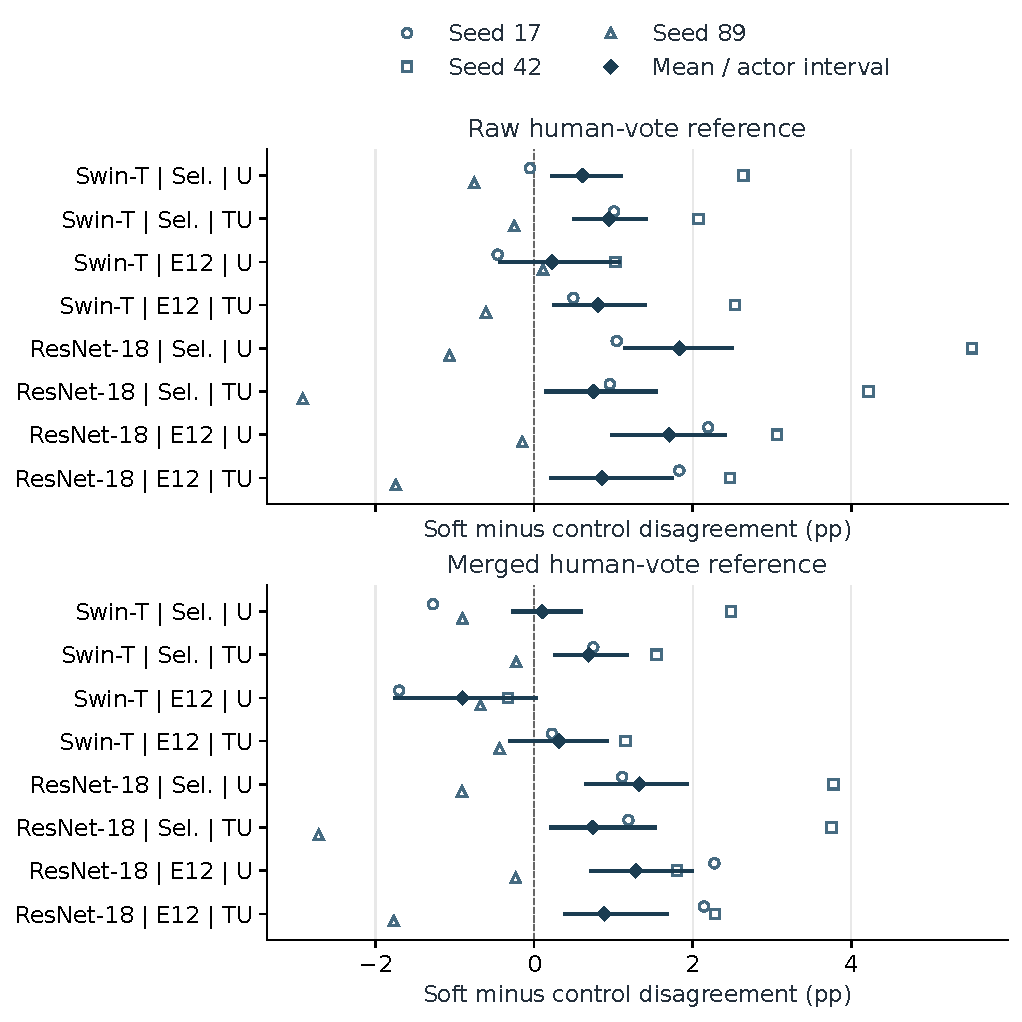
\includegraphics[width=\linewidth]{submission_reader_2026_10_13/source/figures/ExternalContrasts.pdf}

\caption{External disagreement differences at 80\% MSP coverage, using separate model rankings. Hollow symbols show all three paired seed contrasts; the diamond and bar show their mean and conditional 95\% actor-cluster interval. Vertical offsets separate the seeds. Sel.: selected checkpoint; E12: fixed-epoch checkpoint; U: Uniform; TU: Tie-Uniform. Both panels share the horizontal scale; negative favors Soft. Intervals describe actor-sampling sensitivity for these fitted pairs and votes, not uncertainty over new seeds, raters or populations. Zero denotes equal mean disagreement, not equivalent predictions or accepted sets}\label{fig:external}\end{figure}

\begin{table}[htbp]
\caption{Principal external risk accounting: validation-selected Swin-T, means across three seeds (\%). Components use the same population as total risk}\label{tab:externalaccounting}
\centering\small\begin{tabular}{lllrrrr}\toprule
Population & Supervision & Ref. & Risk & Unsup. & Ambig. & Excess\\\midrule
All eligible & Soft & Raw & 71.06 & 11.90 & 16.81 & 42.36\\
All eligible & Uniform & Raw & 70.81 & 11.90 & 16.81 & 42.11\\
All eligible & Soft & Merged & 64.84 & 3.14 & 20.23 & 41.47\\
All eligible & Uniform & Merged & 64.81 & 3.14 & 20.23 & 41.44\\
80\% MSP & Soft & Raw & 68.37 & 14.00 & 16.61 & 37.76\\
80\% MSP & Uniform & Raw & 67.75 & 13.58 & 16.59 & 37.58\\
80\% MSP & Soft & Merged & 60.72 & 3.31 & 20.78 & 36.64\\
80\% MSP & Uniform & Merged & 60.62 & 3.30 & 20.57 & 36.75\\
\bottomrule\end{tabular}\par\smallskip
All eligible: 1,440 clips per state. 80\% MSP: 1,152 independently ranked clips per state. Unsup. is unsupported vote mass; Ambig. is supported ambiguity. All-eligible components are not substituted for accepted-set components. Rounding can prevent displayed components from summing exactly.\par
\end{table}

The risk accounting identifies excess disagreement as the largest component both across all eligible clips and at 80\% MSP coverage (Table~\ref{tab:externalaccounting}). For validation-selected Swin-T Soft under the raw reference, the all-eligible excess is 42.36 percentage points, compared with 11.90 points of unsupported vote mass. Missing output categories alone therefore do not explain the poor transfer. The decomposition describes disagreement rather than its cause, and accepted-set components must be read on their own population rather than substituted from all-eligible averages.

The post hoc diagnostics show that neutral dominates accepted predictions in all three validation-selected Swin-T seeds: 67.0--70.0\% for Soft and 62.7--68.3\% for Uniform. The supplementary vote-weighted matrices and temporal summaries retain all six principal matrices and all eight temporal bins. Neutral probability is highest in the first bin and falls toward the middle, while frame-to-clip argmax agreement also varies across bins. These patterns describe the frozen outputs; they do not establish a cause of transfer failure or measure frame accuracy, since the human judgments apply to whole clips.

Online Resource 8 retains all 36 external states, category frequencies, raw-reference vote mass, raw/merged matrices and temporal summaries. The supplementary score/coverage and fixed-image comparisons provide the complete sensitivity results without changing the primary external comparison.



\FloatBarrier
\section{Discussion}
The results distinguish agreement with the crowd-vote distribution from disagreement among accepted category predictions. Distributional supervision improves the former across the tested source-dataset configurations, but its selective advantage does not persist across both backbones. Fixed-image comparisons further show that the predictor ordering depends on the accepted set. These findings answer RQ1 by qualifying the primary Swin-T advantage: distributional distance and selective risk describe different aspects of performance and cannot be treated as interchangeable evidence of improved recognition.

This distinction develops the evaluation question raised by prior distribution-based FER studies. FER+ and crowdsourced affective supervision established the value of retaining human response distributions rather than treating all disagreement as labeling error \cite{barsoum2016ferplus,washington2021crowdsourcing}. The present controls narrow the interpretation of a hard-versus-soft comparison by preserving dominant target probabilities and tied maxima. They show a smaller selective advantage than the hard-target comparison while retaining a consistent distributional advantage. That pattern supports evaluating both outcomes, but the controls still differ in entropy and aggregate class proportions. The experiment compares these specified target representations rather than isolating the contribution of minority-category identity.

The primary selective effect also warrants attention to scale. A difference of 0.38 pp across 2,620 accepted images corresponds to about 9.9 fewer expected disagreements with a vote drawn from the observed annotations, not 9.9 corrected images. Losses are fractional and the accepted identities differ. For RQ2, the fixed-image analysis explains why each model's own-ranking risk alone is insufficient: prediction quality on a specified accepted set and the composition of that set contribute jointly to the reported outcome. Reference-specific F1 and unsupported-category accounting add two further requirements for interpretation---the label reference and the complete annotation vocabulary must be explicit.

The confidence-score and transfer checks delimit the scope of the selective result for RQ3. Mean differences remain backbone-dependent under the three probability-only scores, and some individual seed comparisons change direction. This extends the connection between annotation disagreement and selective evaluation studied in Crowd-Calibrator \cite{khurana2024crowd}, while leaving learned rejection methods such as SelectiveNet outside the implemented comparison \cite{geifman2019selectivenet}. On RAVDESS, the ordering also depends on the fitted checkpoint and on whether calm and neutral responses are merged. The external diagnostics identify substantial excess disagreement and neutral-dominated predictions, but do not assign a causal explanation to capture conditions, population or temporal aggregation.

Finally, the calibration-transfer results distinguish a nominal risk target from achieved risk. Greater coverage at an empirical threshold is not an equal-risk advantage when the transferred risks differ. The more conservative comparator makes its coverage cost explicit, without verifying that its assumptions hold in deployment. This is consistent with the distinction between confidence scores and calibrated probabilities \cite{guo2017calibration}. Together, the findings motivate a coherent evaluation practice: compare matched supervision targets, report distributional and selective outcomes separately, examine identical accepted sets, specify the annotation reference and vocabulary, and present achieved risk alongside coverage. The conditional intervals quantify sampling sensitivity for the retained fits and observed annotations; they do not establish a general ordering over future training seeds, raters or populations.


\subsection{Limitations and scope of inference}
The principal limitation is adaptive development on one image source. FER+ reannotates FER2013, and earlier PrivateTest outcomes informed subsequent phases; neither the isolated within-source test nor exploratory score sensitivity restores an untouched prospective image evaluation. RAVDESS adds a different media source under a locally frozen plan, but its selection followed known internal findings and annotation metadata. The resulting 24-actor acted-video evaluation tests transfer after changing the prediction unit from image to clip through uniform frame averaging. It is neither an independent static-image training replication nor a naturalistic messaging sample. Pixel and perceptual-hash screening address specific overlap routes rather than all identity or near-duplicate leakage, while external intervals remain conditional on the observed actors and votes. Generalization beyond these populations is unresolved.

Three paired seeds per backbone and a fixed 12-epoch budget also limit optimization claims. Fixed-epoch sensitivity addresses one stopping decision without establishing convergence or robustness to every selection criterion. Grayscale preprocessing, small images, architecture and supported-vote weighting can influence the comparisons. Although two backbone families are examined, the study does not evaluate a learned selector, an independent vote-annotated static-image source or an expanded-vocabulary model. The controls therefore address specified alternative explanations rather than all mechanisms underlying the differences.

Target construction and vocabulary impose further interpretive limits. Uniform preserves the largest training-target probability but generally changes entropy and aggregate class marginals, so its comparison with Soft does not isolate the causal role of alternative-category identities or establish that full distributions are necessary. Tie-hard addresses the fixed tie-breaking convention rather than every possible hard-label construction. Likewise, annotation floors depend on the finite panel, available categories and missing context; they are not fixed properties of a person or image. Adding output categories could change the available-category floor, but supported-mass stratification diagnoses the current vocabulary rather than testing that intervention.

The benchmark population also differs from faces captured during message composition. Lighting, pose, occlusion, accessories, camera quality and detector failures may alter predictions and rejection behavior, and demographic or cultural variation was not evaluated. Consequently, the application remains outside the validated scope: the study provides no mobile-efficiency assessment, runtime error bound, participant findings, survey ratings or interpersonal conclusions. The prototype's unvalidated communication role and sender controls are documented with its implementation rather than used to support the empirical findings.

Finally, the historical preprint's manual-relabeling scores are excluded because their curation records and checkpoints were not retained. The new findings use traceable public annotations rather than a claimed reproduction of that process; Online Resource 1 documents the historical provenance separately. Independent static-image evaluation and an appropriately reviewed communication study remain distinct future work, neither of which is supplied by the external acted-video transfer test.

\section{Conclusion}
Supervision with supported-category vote distributions improves agreement with the complete annotation distribution across the tested source-dataset configurations, but does not provide a consistent advantage in selective category disagreement. The primary validation-selected Swin-T comparison favors Soft over the dominant-confidence-matched control, whereas the adaptive ResNet-18 checks do not confirm that selective advantage. Comparisons on identical images depend on the accepted set, and external comparisons vary with training seed, checkpoint state and annotation reference. The resulting contribution is an evaluation of these dependencies through matched targets, fixed-image comparisons and complete-vocabulary risk accounting. Reporting distributional agreement separately from selective disagreement, and achieved risk separately from nominal targets, provides a more precise interpretation of crowd-supervised facial-expression prediction within the scope of these experiments.



\backmatter
\section*{Statements and Declarations}
\noindent\textbf{Funding.} No funds, grants, or other support were received for preparation of this manuscript.

\noindent\textbf{Competing interests.} The authors declare no competing interests.

\noindent\textbf{Author contributions.} Gunjan Kumar Mishra conceived the prototype and led manuscript preparation. Bijaya Ghimire contributed to implementation, experimental design, and manuscript revision. Badri Raj Lamichhane supervised the work, contributed to methodology review, interpretation, and manuscript revision, and serves as corresponding author. Alan Shah contributed to literature review and code testing. All four authors approved the scientific content, authorship arrangement and declarations.

\noindent\textbf{Ethics approval.} This study comprises secondary analysis of existing benchmark images, video-only speech clips and annotations, together with software tests. No institutional ethics approval or exemption determination was obtained.

\noindent\textbf{Consent to participate.} No participants were recruited and no new human ratings were collected for the analyses reported here. The RAVDESS publication reports consent and ethics review for its original collection; this does not constitute approval of the present analysis. Photograph-level consent records for FER images were not independently verified.

\noindent\textbf{Consent for publication.} No identifiable facial photograph is reproduced. Interface illustrations contain synthetic text and no participant images.

\noindent\textbf{Data availability.} Acquisition records for FER2013 \cite{goodfellow2013fer} and official FER+ annotations \cite{barsoum2016ferplus}, immutable hashes, role assignments, and sample-level model probabilities are supplied in Online Resource 1. The consolidated Online Resource 1 also supplies the exploratory confidence-score protocol, code, all score/coverage summaries and input hashes. Images are not redistributed. The full ten-category FER+ annotations are retained for auditing the reported metrics. RAVDESS original S5 human responses and official media are available from its primary publication and Zenodo record \cite{livingstone2018ravdess}; Online Resource 8 retains derived nine-category counts, model probabilities and integrity records, without redistributing video or facial images.

\noindent\textbf{Code availability.} The accompanying Online Resource 1 supplies within-source experimental, analysis and application code, tests, environment records, retained predictions and scientific provenance. Online Resource 8 supplies the external protocol, amendment, predictions and post hoc diagnostic code and exports. Online Resources 2--6 contain the 30 Swin-T selected and epoch-12 checkpoints; Online Resource 7 contains all 18 ResNet-18 checkpoints. The resource map supplies checksums and executable numerical-replay commands without requiring restricted media. Earlier code is at \url{https://github.com/mgunjan67/crowd-supervision-selective-fer}; that release does not replace the current accompanying resources. Automated regeneration is internal verification, not external replication.

\noindent\textbf{Preprint statement.} An earlier version appeared on TechRxiv as ``Typing with Emotions: Facial Expression Recognition and Embedding in Text Messages,'' version 1, \url{https://doi.org/10.36227/techrxiv.175416003.30236370/v1}. This revision excludes participant evidence and unverifiable historical performance claims, corrects implementation descriptions, and supplies newly documented experiments. It does not claim to reproduce the historical curation procedure.

\noindent\textbf{Supplementary information.} Online Resource 1: code, all four adaptive protocols, acquisition and split manifests, per-seed predictions and results, supplementary diagnostics, and historical provenance. Online Resources 2--7: all 48 selected and fixed-epoch inference checkpoints, grouped by backbone and supervision condition, with checksum manifests. Online Resource 8: frozen RAVDESS protocol, clip/frame probabilities, complete external ledgers, source hashes and independent verification; no media or duplicate weights.

\FloatBarrier
\bibliography{submission_reader_2026_10_13/source/references}
\end{document}
